\chapter{SUPPORTING GUIDANCE IMPLEMENTATION AND VALIDATION}
\label{app:guidance-support}
This appendix preserves the engineering detail needed to reproduce the apparatus and examine delivery faults. Its state-machine design, memory, provider comparisons, and diagnostic examples support the self-similar voice study; they do not add participant conditions or establish the benefit of any guidance policy. Implemented behavior, proposed checks, and missing evidence retain the status stated in each section.

\section{Short-Term Interaction Memory}
To give guidance continuity, the system maintains two short-term memories. A spatial history tracks turning progress and supports cues that return the participant to the target, while a speech-decision memory records what the system actually said and how the guidance state changed. Each speech entry stores its relative age, context, and whether playback completed or was interrupted; each state entry stores the prior and current states and the reason for the transition. The speech and transition lists each retain at most four entries, and snapshots sent to Jev exclude entries older than 15 seconds. This bounded recent context is related to the context-management motivation of EmBARDiment~\cite{bovo2025embardiment}, although the current implementation does not use its object-admission or dropout policy. The spatial history, by contrast, retains up to three seconds or 384 target-relative gaze observations and is cleared on invalid evidence, source changes, or observation gaps longer than 100~ms. These limits are engineering settings, not validated fixation or blink thresholds.

The interaction gates are likewise engineering settings. Gaze-vicinity confirmation currently requires 100~ms of valid qualifying evidence; invalid evidence resets its entry timer, and reacquisition after a spoken confirmation requires 150~ms of valid gaze away. These gates do not admit objects to speech memory, and missing gaze is not counted as observed dwell. Both memory types are cleared whenever guidance resets and are copied before each asynchronous request. The memory is therefore deliberately scoped to the current task: it neither builds a persistent participant profile nor attempts to infer unobserved mental states.

Figure~\ref{fig:bounded-memory} shows which recent evidence accompanies an asynchronous request. Its time limits bound the software context and must not be interpreted as estimates of human short-term memory.

\begin{figure}[htbp]
\centering
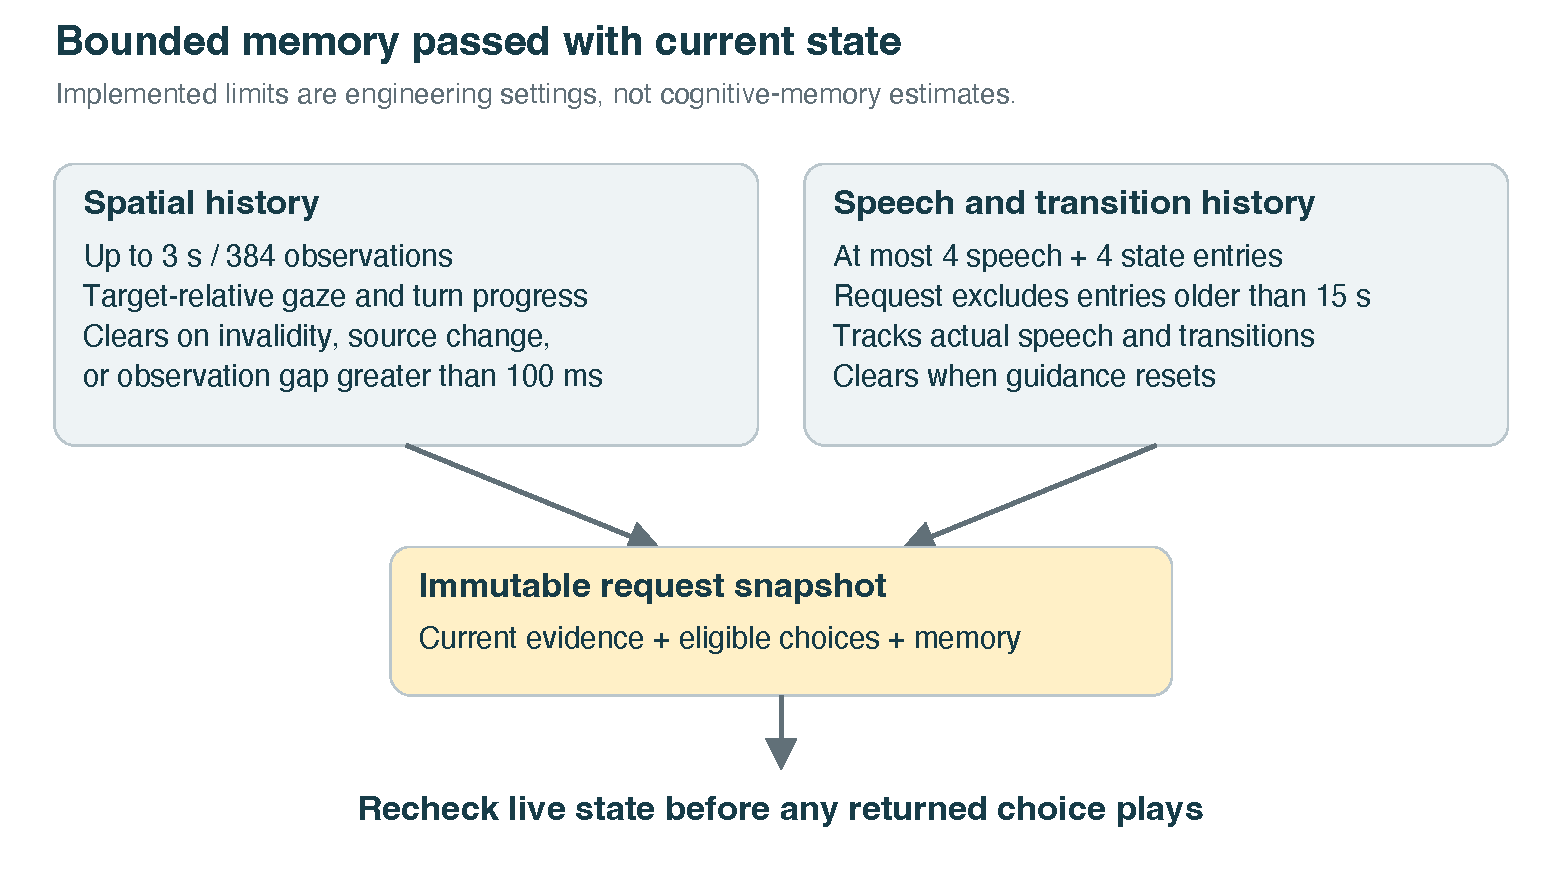
\includegraphics[width=\linewidth,alt={Spatial history and recent speech and state history are copied into a request and checked against current state before playback.}]{figures/bounded-memory.pdf}
\caption[Bounded spatial and speech memory]{Implemented memory limits and snapshot boundary. Spatial history and speech/state history have different retention and reset rules. A copied request preserves its original context, while playback still requires a fresh state check.}
\label{fig:bounded-memory}
\end{figure}


\section{Ownership and State Transitions}
The central guidance machine is a plain C\# object, while Unity MonoBehaviours connect it to tracked devices, scene objects, and audio; this arrangement separates deterministic state transitions from engine callbacks. Responsibility during a session is divided among three components. The round manager owns readiness, trial onset, completion, pause intervals, and block progression; the guidance machine owns the interpretation of evidence during search; and the speech scheduler owns pending requests, cancellation, and playback admission. The application is thus coordinated through distinct responsibilities rather than a single global state variable.

A state label is useful only when it is accompanied by its evidence. A refining state indicates that guidance has entered the target wall, but it does not prove that the eyes intersect the target object; likewise, an acquired state can reflect qualified vicinity evidence without implying that a trigger selection occurred. The viewer therefore presents state transitions alongside gaze-hit, vicinity-candidate, controller-hit, and playback records, so that an apparent disagreement can be inspected rather than the label being assumed to be complete ground truth.

\begin{table}[htbp]
\centering\caption{Guidance responsibilities and evidence boundaries.}
\small\tagpdfsetup{table/header-rows={1}}
\begin{tabularx}{\linewidth}{@{}p{0.22\linewidth}XX@{}}\toprule
Component & Owns & Does not establish \\\midrule
Observation adapters & Validity, poses, ray hits, source timing & Recognition or fixation \\
Guidance machine & Stage, eligible action, bounded history & Correct trigger selection or conscious recognition \\
Jev decision provider & Choice among eligible phrases; speak or wait & New target identity or unchecked geometry \\
Speech scheduler & Current-state check, pacing, cancellation, start & Acoustic arrival at the ear \\
Round manager & Readiness, reveal, selection, pauses and blocks & Independent validation of gaze accuracy \\
Trial Review & Reconstruction from saved evidence & Missing observations between recorded samples \\\bottomrule
\end{tabularx}
\end{table}

The usual path runs from turning toward a wall, through refinement within it and gaze acquisition of the target, to preparation for selection. This is not, however, a mandatory one-way chain: participants can overshoot, revisit a wall, point before gaze qualifies, or lose tracking. The implemented state families represent these returns, and release testing must verify them without the system repeatedly announcing a new arrival whenever the participant looks upward on the same wall. Invalid or stale evidence suspends new gaze-dependent decisions rather than being treated as a departure.

Figure~\ref{fig:guidance-states} summarizes the state families. The arrows show a common progression rather than compulsory transitions: correct right-trigger selection can complete an active trial without a preceding spoken gaze or pointing acknowledgment.

\begin{figure}[htbp]
\centering
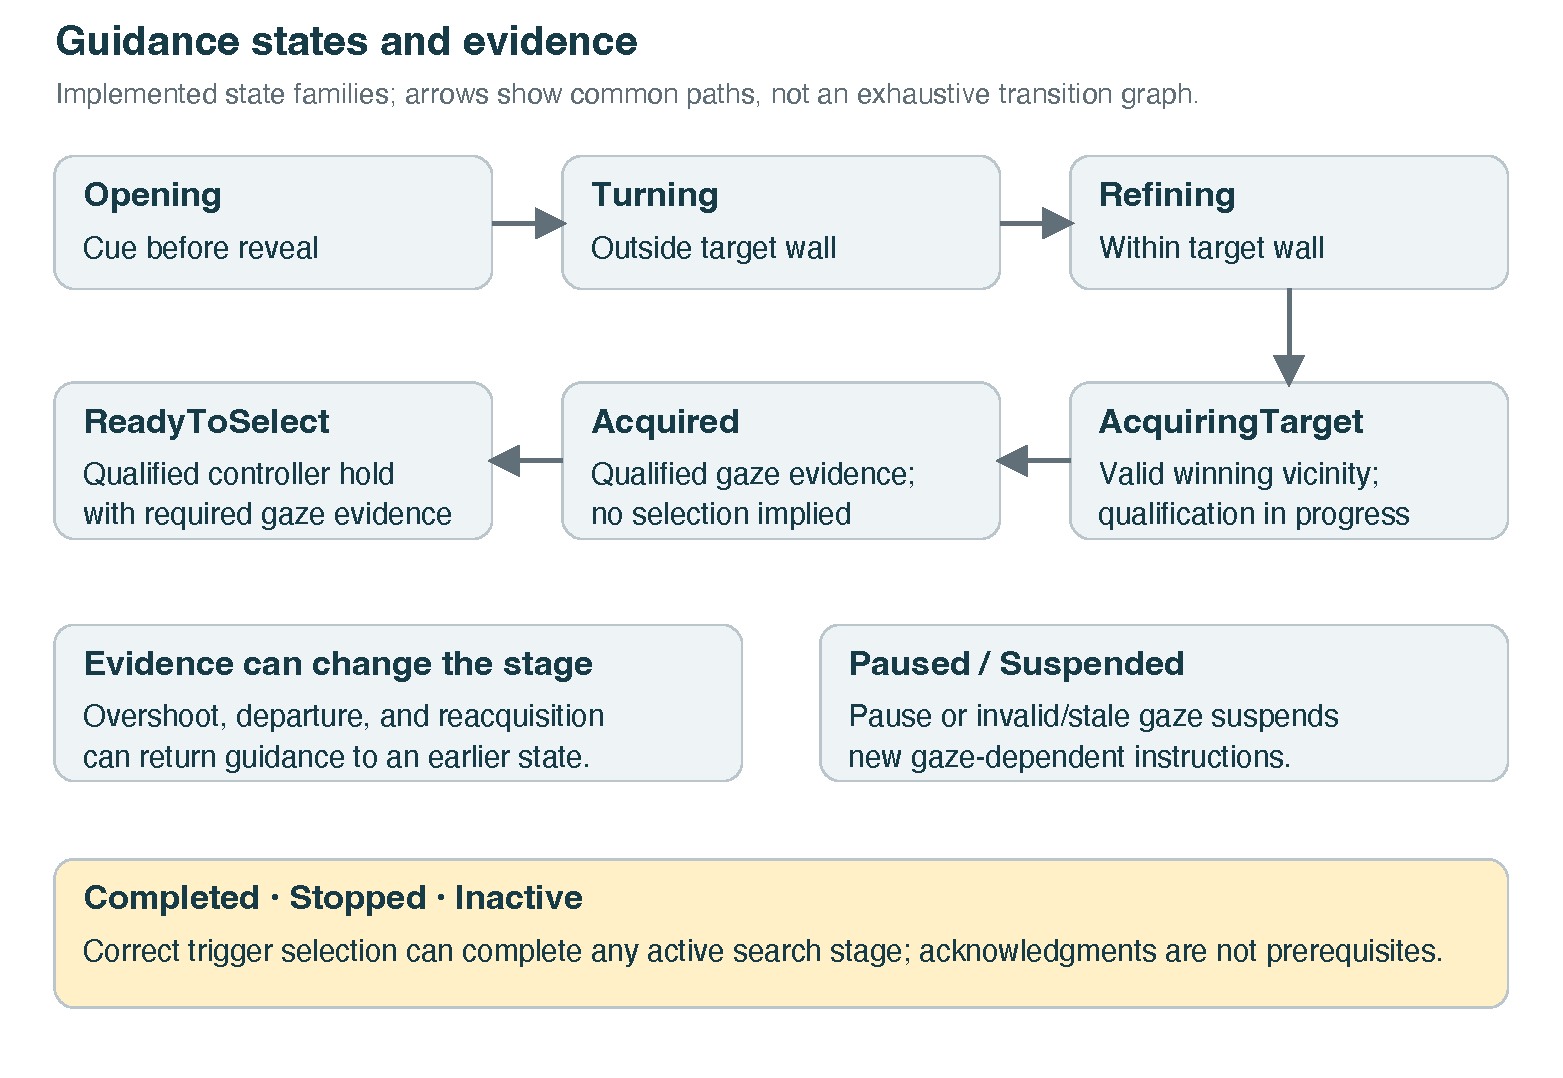
\includegraphics[width=\linewidth,alt={Common path from opening through turning and refinement to acquisition and readiness, with pause and suspension and independent trigger completion.}]{figures/guidance-states.pdf}
\caption[Guidance states and evidence-dependent transitions]{Implemented guidance state families. Turning, refining, acquisition, and readiness are evidence-dependent interpretations. Tracking loss, pauses, target departure, and reacquisition can change the path. Trial completion remains owned by the round manager.}
\label{fig:guidance-states}
\end{figure}


\section{A Worked Guidance Sequence}
Consider an illustrative target near the wall opposite the starting cross, with a rightward offset or the documented backward-turn tie rule. The opening cue may say that the object is to the right while objects remain hidden. Once search begins, progress cues can acknowledge continued rightward turning. On stable entry to the target wall, assistance can move to within-wall refinement, such as looking lower and slightly left. The reference for that refinement must be the recorded gaze geometry and local target relation, not a neighboring object's apparent screen position.

If the participant passes the target, recent spatial history can support a return cue. If the participant instead looks near the target long enough, a gaze acknowledgment becomes eligible, and if the controller is already intersecting the target, away-directions are suppressed immediately. A qualified pointing acknowledgment can then identify controller evidence, and a right-trigger press can complete the trial. This example illustrates intended transitions; it is not a measured trajectory or evidence that all people follow this sequence.

\section{Asynchronous Decisions and Cancellation}
Each cloud request receives a snapshot rather than a live reference to mutable state, comprising current evidence, relevant geometry, speech status, and bounded recent history. Because a response can become stale if the participant moves, tracking changes, the voice changes, a pause begins, or the trial ends, the scheduler checks these conditions again before playing the chosen clip. A valid answer to an old question is not necessarily a valid instruction now.

Prepared audio removes synthesis from the immediate hint path, but it does not remove network latency from cloud choice. Time-sensitive qualified feedback can therefore use local admission without waiting for another Jev decision, whereas ordinary hints can wait for a phrasing choice within bounded scheduling rules. Interruption policy balances urgency against comprehensibility, since finishing a short useful phrase may be preferable to cutting it at an awkward boundary. The documented implementation uses a 150-ms fade as a playback technique, not a guarantee of natural conversation.

Experimental policies that allow Jev broader action choice must be versioned separately from the participant policy. Replaying the same observations through multiple policies can compare decision latency and admissibility, but it cannot show how a participant would have moved after hearing a different cue. The participant release will therefore need one frozen policy and a manifest of thresholds, phrase library, Jev provider/model identifier, version, and available sampling settings. Whether the provider sees voice-condition identifiers must also be verified against the frozen payload. This draft does not assume condition-blind decisions, and that audit will distinguish voice-related cancellation keys from information actually transmitted to the provider.


\section{Operational Configuration and Reproducibility}
The method must preserve the conditions under which a decision was made, not only the selected phrase. A reproducibility record will bind the application revision to the gaze-source configuration, state-machine gates, phrase semantics, provider request contract, voice library, and instrument versions. Without that binding, a later replay can use the same target positions while silently changing the policy that produced the original speech.

Appendix~\ref{app:decision-contract} documents a code-inspected decision contract and a proposed release manifest. The inspection covers the recovered working implementation on October 23, 2026; it is not evidence that this working revision was merged, installed, or used by participants. In the inspected request builder, ordinary phrase selection uses a named choice question with eligible texts as keys in a criteria object, a combined request also asks whether to transmit, and returned selections must match the submitted candidates. The intended playback boundary additionally requires current-evidence rechecks, and the appendix distinguishes the inspected request and state code from release-wide checks still to be verified. Exact request and response records should accompany future claims about model behavior.

The application and external services have different reproducibility limits. Local geometry can be rerun from source and input fixtures, whereas a hosted model alias may resolve to a changed service even if its string is unchanged, and prepared audio can retain the original output while its provider's current synthesis changes. Accordingly, the study record will identify both configuration and realized outputs where permitted: actual candidate sets, returned choices, delivered clip identifiers, and playback events. A credential is never part of the research manifest.

No best-performing provider or autonomous policy is established by this manuscript. The offline comparison described below is a route to testing such alternatives. It must preserve the distinction between deciding what a model would say on a replayed trajectory and observing how a participant responds to that speech.

\section{Why Sequence Evaluation Is Necessary}
A phrase can be geometrically admissible in isolation and still be poor guidance in sequence. Repeating a direction immediately after it was delivered can be unnecessary, and a correct downward cue can become obsolete once the controller reaches the target. Likewise, a gaze acknowledgment can arrive late after multiple model waits even though each individual response was well formed. Evaluation must therefore inspect recent state, actions, and actual speech around the event.

Deterministic checks will first establish whether the evidence supports an action, distinguishing gaze confirmation, controller confirmation, and trial completion. A model judge may then use that evidence to assess the appropriateness of wording, timing, repetition, and interruption. Its ratings remain advisory: they do not represent human-perceived correctness, and they cannot convert an incompletely logged episode into a known success or failure.

\section{Paired Policy Pilots}
Paired pilots will feed identical recorded states and scripted trajectories to the baseline and candidate policies. The scenario set includes large turns, wall entry, vertical refinement, overshoot, gaze on target with the controller elsewhere, controller on target with nearby gaze, overlapping vicinity regions, blinks, stale tracking, pauses, and delayed model responses. Audio occupancy and readiness must also be represented so that playback admission can be compared fairly.

The candidate-policy comparison may include small, medium, and full eligible phrase sets. Full eligible means all choices that still satisfy hard geometry and validity requirements; it does not mean handing the model an unfiltered catalog and ignoring physical constraints. Provider support and exact candidate counts will be recorded. Experimental policies will remain outside participant builds until their results justify a controlled change.

Replaying an observed trajectory is a counterfactual engineering test. The original participant did not hear the alternative sequence, so the replay cannot demonstrate that the alternative would have reduced their search time. Scripted trajectories provide reproducible edge cases but are not measured human behavior. Both are useful for identifying faults before a wearer pilot.


\subsection{Development Cases and an Untouched Evaluation Set}
\textbf{Protocol proposal.} The engineering evaluation will maintain three explicitly labeled sources of cases: scripted fixtures that exercise known transitions and fault conditions, a development corpus of recorded sequences used to identify faults and tune policy, and a separate evaluation corpus held out from those tuning decisions. At this stage, no frozen split, sample count, or completed held-out score is claimed.

The split must occur at a level that prevents closely related observations from appearing on both sides. Adjacent requests from the same confirmation episode cannot be separated into development and evaluation as if they were independent cases. Where feasible, whole sessions, and participants when repeated sessions exist, will be assigned together. The release record will enumerate included sessions, duplicate checks, exclusions, and the moment at which the policy was frozen. It will identify each corpus as scripted, developer, pilot, or participant data. Participant-derived sequences will be replayed through hosted providers only where consent and data-handling terms permit. Previously inspected development runs cannot later be described as untouched evaluation data.

For a model-assisted judge, a human-reviewed calibration subset will define how the rubric is applied. Reviewers will see the same recorded evidence and mark unsupported conclusions as unknown. Disagreements will be retained, discussed, and used to clarify the rubric before evaluating the held-out set. A model judge's agreement with this subset is not a measure of participant perception. Repeatedly tuning the judge against the evaluation set would invalidate its held-out role just as repeated policy tuning would. The proposed review will mask policy labels and voice-condition identifiers where they are not required to interpret the evidence, while recording any residual clues that prevent effective blinding. Human--human and judge--human agreement statistics will be specified with the rubric before evaluation; unknown cases will retain their own reported count rather than silently disappear from denominators.

\subsection{Controlled Policy Comparisons}
Table~\ref{tab:policy-pilots} defines the comparison roles discussed during development. The table is a prospective evaluation design, not a report of measured winners. Candidate-set size and decision autonomy are separate manipulations: widening eligible wording while holding the action policy fixed does not test the same question as allowing the provider to choose a different action family.

\begin{table}[htbp]\centering
\caption[Proposed policy comparison and safeguards]{Engineering comparison roles. All policies retain valid input interpretation and explicit logging; experimental variants do not enter participant sessions on the basis of this table.}
\label{tab:policy-pilots}
\small\tagpdfsetup{table/header-rows={1}}
\begin{tabularx}{\linewidth}{@{}p{0.24\linewidth}XX@{}}\toprule
Policy role & Decision authority & What the comparison can test \\\midrule
Constrained Jev with local feedback & Local eligible action; provider chooses wording and speak/wait; qualified local feedback can bypass a new request. & Reference behavior and delivery delay under the shared scheduler. \\
Jev-led with local overrides & Provider considers meaningful eligible actions using state/history; local geometry, qualification, and final admission remain binding. & Whether broader choices improve sequence appropriateness without unacceptable delay. \\
Provider-led replay probe & Provider receives broad state and action choices; overrides are recorded as shadow checks rather than used to declare the model correct. & Unsupported choices and response timing offline. This is not an approved participant policy. \\\bottomrule
\end{tabularx}
\end{table}

The ordinary inspected request contract accepts two to five candidate phrases. A full-eligible-set experiment therefore requires an explicitly versioned test adapter when more than five candidates are eligible; this draft does not claim that the inspected request wrapper supports an arbitrary catalog size. Each pilot will log its actual candidate count, serialized payload size, request path, and model identifier. Small, medium, and full sets will be defined before execution rather than assigned favorable labels after observing results.

Paired execution will hold input timestamps, target geometry, validity, audio availability, and scoring rules constant. Model repetitions and execution order should be prespecified to expose stochastic variation and service-time effects. Independent request calls do not eliminate order-related network or server-load variation. Results will distinguish per-call transport measurements from whole-sequence behavior and will not substitute an average request latency for confirmation delivery time.

\section{Metrics and Episode Definitions}
For each policy, the report will summarize qualification-to-software-playback latency with median, 95th percentile, maximum, and count beyond a stated engineering threshold. The threshold must be declared before comparison and distinguished from a perceptual or clinical criterion. Episodes, rather than repeated requests within an episode, will be the denominator for delayed confirmations.

Jev request latency, failures, timeouts, calls per trial, cancellations, and late responses will be reported separately. A provider timeout can lead to a timely local fallback, while a successful provider response can still arrive too late for the current state. Provider reliability and delivered guidance reliability therefore require different measures.

Wrong-direction and stale hints will be labeled only when the available evidence shows that the instruction is unhelpful toward the task; a different but valid phrase is not automatically wrong, and missing evidence remains unknown. Judgments about repetition, unnecessary speech, excessive silence, and interruption appropriateness likewise require context beyond a sign check on an angle.

\section{Illustrative Failure Analysis}
An ordering failure can occur when a correction is queued before the controller reaches the target, and several distinct mechanisms could produce it. If playback checks use the older snapshot, the correction can play immediately before a pointing acknowledgment. Alternatively, the controller hold may not yet have qualified, leaving the ordinary-direction policy active during the hold, or action priority may admit a lower-priority cue despite newer pointing evidence. These causes require different fixes, yet they cannot be distinguished from the spoken text alone.

The intended correction is to suppress contradictory away-directions as soon as valid controller-on-target evidence is present, while retaining the independent qualification timer for the spoken pointing acknowledgment. A final playback check must repeat the suppression after any asynchronous wait or audio fade. If the controller leaves the target before qualification, no pointing acknowledgment should be emitted merely because the earlier request was valid.

A separate reference-frame problem arises when an object appears higher than a highlighted neighbor but the instruction says to look lower. If the instruction is calculated relative to the current eye ray, which could lie above both objects, the phrase can be geometrically consistent yet confusing because the highlight suggests a different reference object. Diagnosis therefore requires the recorded gaze ray, object positions, highlighted candidate, and playback time; it must not rely only on the review camera's screen-space layout.

These examples are diagnostic categories drawn from the development history. This appendix does not report their incidence or claim they have all been eliminated in a frozen participant build. The acceptance matrix in Appendix~\ref{app:scenarios} defines evidence required to make those claims.


\subsection{A Proposed Failure Taxonomy}
Table~\ref{tab:failure-taxonomy} classifies potential faults by where evidence is lost or acted on incorrectly. These categories organize review; they are not observed error rates. More than one category may contribute to an episode. When the trace does not establish a causal stage, the result remains unresolved rather than being assigned to Jev by default.

\begin{table}[htbp]\centering
\caption[Failure categories and diagnostic evidence]{Proposed sequence-review taxonomy. A label requires evidence from the relevant stage, and does not imply a frequency estimate.}
\label{tab:failure-taxonomy}
\small\tagpdfsetup{table/header-rows={1}}
\begin{tabularx}{\linewidth}{@{}p{0.24\linewidth}XX@{}}\toprule
Category & Diagnostic evidence & Example distinction \\\midrule
Observation or geometry & Validity, source age, coordinate frame, gaze ray, object transforms & Wrong spatial input versus a correct cue calculated from that input. \\
State or qualification & Gate timers, transition cause, controller hit, vicinity winner & Immediate pointing evidence versus qualified pointing acknowledgment. \\
Decision or context & Exact request snapshot, candidates, history, response & Unsupported choice versus an admissible alternative wording. \\
Scheduling or delivery & Cancellation, queue, final check, clip readiness, playback start/end & A valid old proposal that becomes stale before it speaks. \\
Interaction or reference & Visible highlight, task state, phrasing, recent speech & A geometric direction that is confusing relative to the highlighted neighbor. \\
Recording or scoring & Clock mapping, missing events, join version, episode identity & Missing evidence or duplicate counting versus a demonstrated runtime fault. \\\bottomrule
\end{tabularx}
\end{table}

\subsection{Worked Sequence Diagnosis}
The following cases are constructed examples, not participant observations. Their purpose is to show what evidence would justify a finding. Let $t_q$ be the first supported qualification and $t_p$ the actual software playback start, as defined in Chapter~\ref{ch:measurement}.

\begin{enumerate}
\item \textbf{A direction becomes stale during a controller hold.} A downward cue is eligible at request time. Before its response arrives, the tracked controller ray hits the target. The hold is not yet qualified, so a pointing acknowledgment would be premature. Under the intended policy, the search direction is suppressed and the hold gate preserved. If the old direction actually plays, the finding concerns admission or scheduling; if it was merely proposed and rejected, it is not a delivered wrong hint.
\item \textbf{Gaze qualifies while the controller remains elsewhere.} Valid winning-vicinity evidence satisfies the gaze gate at $t_q$. A looking acknowledgment is appropriate; a pointing acknowledgment is not. For a policy that routes this acknowledgment through the provider, repeated model waits followed by playback at $t_p$ form one delayed gaze-confirmation episode. Under the reference local-feedback path, a comparable delay would instead require investigation of scheduling, audio readiness, or delivery. Attribution requires the wait and scheduler records. It cannot be inferred from the final spoken text alone.
\item \textbf{The eyes and a nearby highlight imply different reference points.} The gaze ray is above both a target and a highlighted distractor, but the target is higher than that distractor. A lower cue may be consistent with the gaze ray while appearing wrong relative to the highlight. This warrants a reference-frame or wording concern, not an automatic wrong-sign label. The review must inspect the state at playback rather than only a screenshot after movement.
\end{enumerate}

For each reported real example, the completed thesis will provide the case-selection rule, a short surrounding timeline, the proposed versus played wording, the governing evidence, and the reason for the label. A few selected examples can explain a mechanism; they cannot establish its prevalence. Frequency claims require the defined evaluation denominator, including unknown and unreviewable episodes.

\section{Interpreting Two-Second Delays}
A two-second delay can contain several different intervals: waiting for qualification, waiting for a model response, an explicit model decision to wait, queued speech, audio readiness, and playback scheduling. Removing a provider wait does not establish that all delays disappear. Conversely, a one-second controller hold is an intentional qualification period, not necessarily a one-second processing fault.

The appropriate test starts from the first supported qualification for the particular event and ends at its actual software playback. A gaze event with a 100-ms gate and a controller event with a one-second hold must not share an undifferentiated origin. The report will retain both first evidence and qualification time so that readers can distinguish intentional gating from added delivery delay. Without a new verified sequence dataset and a wearer or acoustic measurement where required, this draft cannot claim that the roughly two-second delays have been removed.
